% Roameo: agents plan the trip, you make the call. One-slide 2-minute presentation (landscape
% poster, 16:9). Authors: Zhen Lu and Noctis Zhang.
% Built on the Gemini beamerposter theme (https://github.com/anishathalye/gemini, MIT License,
% see LICENSE-gemini.md) with a neutral colour theme (beamercolorthemeroameo.sty).
% Build: latexmk -pdflatex='lualatex -interaction nonstopmode' -pdf poster.tex
%
% The story and the layout follow ../STORY_PLAN.md. Every number comes from the repository: the
% evaluation files in docs/, README.md, the code under backend/, and one real run of the app
% shown in docs/screenshots/03_over_budget_escalation.png. The figures are the poster variants in
% ../slides/figures/ (fig_story_v, fig_system_poster, fig_results_poster, fig_qr).

\documentclass[final,usepdftitle=false,hyperref={pdfauthor={Zhen Lu and Noctis Zhang},pdftitle={Roameo: agents plan the trip, you make the call}}]{beamer}
% Keep the PDF metadata to title and author.
\pdfvariable suppressoptionalinfo 1023
\hypersetup{pdfcreator={},pdfproducer={}}

% ====================
% Packages
% ====================

\usepackage[T1]{fontenc}
% 48 x 27 inches, exactly 16:9, so it projects as one slide and prints as a flyer.
\usepackage[orientation=landscape,size=custom,width=121.92,height=68.58,scale=1.25]{beamerposter}
\usetheme{gemini}
\usecolortheme{roameo}
% Projection needs heavier strokes than the template's Lato Light.
\setsansfont{Lato}[UprightFont=*-Regular, ItalicFont=*-Italic, BoldFont=*-Bold, BoldItalicFont=*-BoldItalic]
\addtobeamertemplate{block begin}{}{\raggedright}
\addtobeamertemplate{block end}{}{\vspace*{-1ex}}
\usepackage{graphicx}
\usepackage{anyfontsize}
\usepackage{fontawesome5}
\usepackage{tikz}
\hyphenpenalty=10000
\exhyphenpenalty=10000
\setlength{\parskip}{0.6ex}

\graphicspath{{../slides/figures/}{../screenshots/}}

\definecolor{accent}{HTML}{C2410C}
\definecolor{ok}{HTML}{4D7C0F}
\definecolor{muted}{HTML}{5F6368}

% ====================
% Lengths
% ====================

\newlength{\sepwidth}
\newlength{\colL}
\newlength{\colC}
\newlength{\colR}
\setlength{\sepwidth}{0.0125\paperwidth}
\setlength{\colL}{0.262\paperwidth}
\setlength{\colC}{0.392\paperwidth}
\setlength{\colR}{0.296\paperwidth}
\newcommand{\separatorcolumn}{\begin{column}{\sepwidth}\end{column}}

\setbeamerfont{block title}{family=\Raleway,size=\Large,series=\bfseries}
\setbeamertemplate{footline}{}
\newcommand{\figcaption}[1]{{\normalsize\color{muted}#1\par}}
\newcommand{\option}[1]{\tikz[baseline=(b.base)]\node[draw=roameoteal, line width=2pt, rounded corners=16pt, inner sep=10pt, text=roameoink] (b) {#1};}

% ====================
% Title
% ====================

\title{Roameo: agents plan the trip, you make the call}
\author{An AI trip planner that does the research and the math, and asks before it goes over your budget}
\institute{Zhen Lu \quad Noctis Zhang \qquad PEAAII AI Applications Hackathon 2026, Agentic AI \qquad October 2026}

\logoright{
\includegraphics[height=7.2cm]{fig_qr.pdf}}

% ====================
% Body
% ====================

\begin{document}

\begin{frame}[t]
\begin{columns}[t]
\separatorcolumn

% ---------------------------------------------------------------- left: the story
\begin{column}{\colL}
  \begin{block}{Alex has \$600 and one sentence}
    \begin{center}
      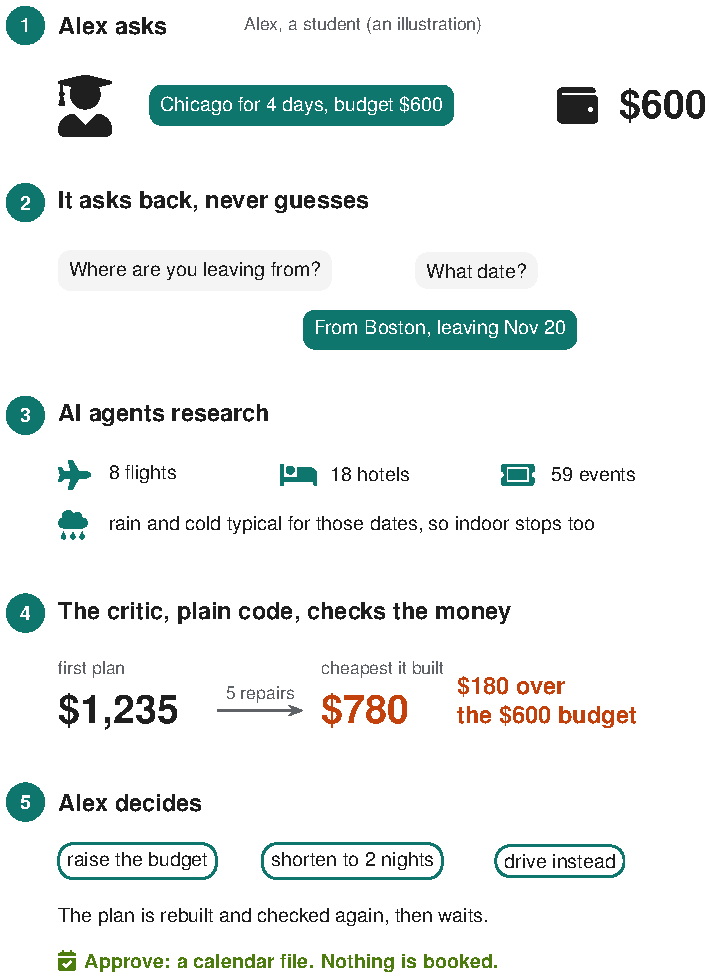
\includegraphics[width=\linewidth]{fig_story_v.pdf}
    \end{center}
    \vspace{0.2cm}

    Words and numbers: \textbf{one real run} of the app, with live flights, hotels and events. Alex is an illustration.

    Built for \textbf{students and budget travellers} on short trips, and for small groups who split the cost.
  \end{block}
\end{column}

\separatorcolumn

% ---------------------------------------------------------------- centre: the moment and the system
\begin{column}{\colC}
  \begin{block}{Over budget? It stops and asks you}
    \begin{columns}[T]
      \begin{column}{0.60\linewidth}
        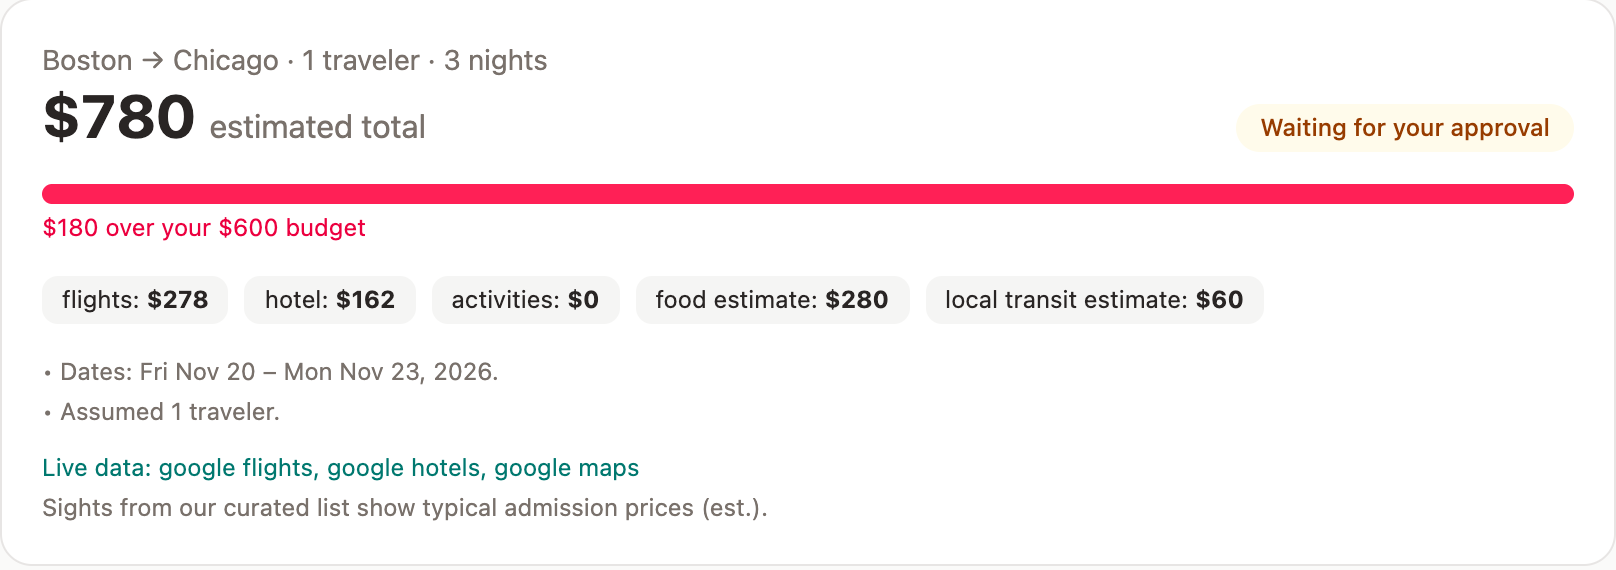
\includegraphics[width=\linewidth]{esc_budget.png}
        \figcaption{Alex's plan in the app: \$180 over the \$600 budget, waiting for approval.}
      \end{column}
      \begin{column}{0.38\linewidth}
        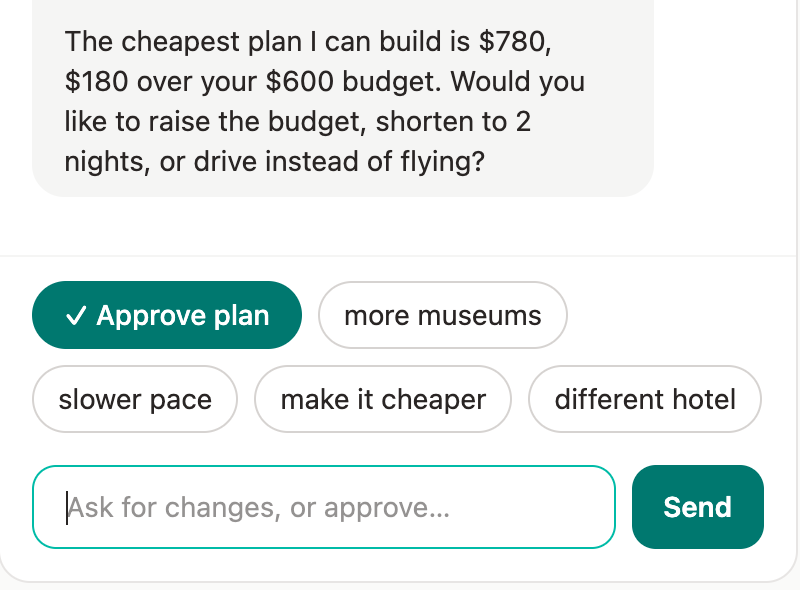
\includegraphics[width=0.9\linewidth]{esc_question.png}
      \end{column}
    \end{columns}
    \vspace{0.3cm}
    {\Large\bfseries\color{roameoink}Your call:}\hspace{0.8em}\option{raise the budget}\hspace{0.5em}\option{shorten to 2 nights}\hspace{0.5em}\option{drive instead of flying}
  \end{block}
  \begin{block}{AI agents gather, code checks the money, you decide}
    \textbf{Why agents, and not one prompt?} Each step depends on the one before: the questions, what the tools found, the price after each repair. The agents choose what to look up, and plain code does the arithmetic.
    \begin{center}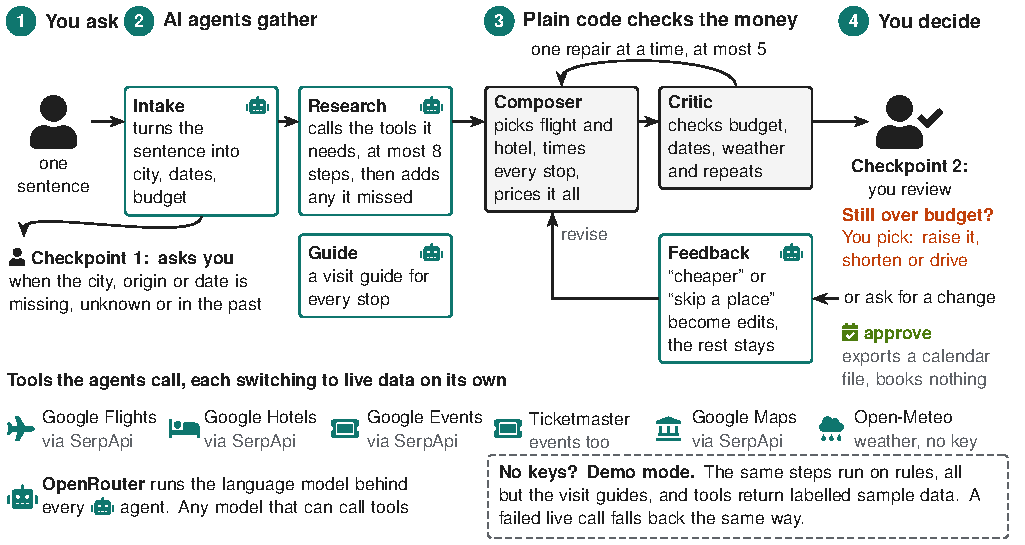
\includegraphics[width=0.96\linewidth]{fig_system_poster.pdf}\end{center}
  \end{block}
\end{column}

\separatorcolumn

% ---------------------------------------------------------------- right: evidence and how to try it
\begin{column}{\colR}
  \begin{block}{All 23 core tests pass in both modes}
    \begin{center}
      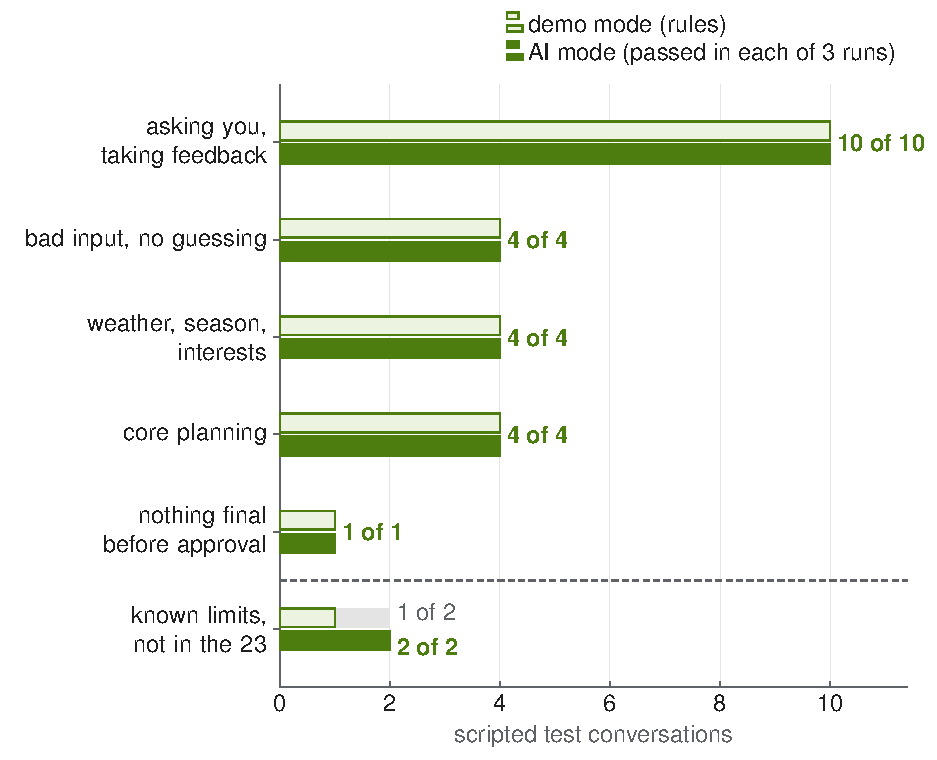
\includegraphics[width=\linewidth]{fig_results_poster.pdf}
    \end{center}
    A test is a scripted conversation with checks on the result, such as \emph{total within budget}: 51 checks in the 23 core tests. AI mode ran 3 times. We wrote the tests, on sample prices, so this is a small, honest check, not a user study.
  \end{block}
  \begin{block}{Try it, deploy it}
    {\color{roameoteal}\faTerminal}\enspace No keys: demo mode on a laptop in about 3 minutes.

    {\color{roameoteal}\faGlobe}\enspace One Render URL, an access code, 60 requests per visitor per hour. If the live demo asks for an access code, ask us.

    {\color{roameoteal}\faKey}\enspace Any OpenRouter model. Each tool switches to live data on its own.

    {Limits: sample data for 7 cities, food and transit are estimates, many events have no price, no user study yet.}
  \end{block}
\end{column}

\separatorcolumn
\end{columns}
\end{frame}

\end{document}
